\documentclass{standalone}

\usepackage{tikz}
\usepackage{amsmath}
\usetikzlibrary{arrows}


\begin{document}
\begin{tikzpicture}[>=latex]
	% Ebene
	%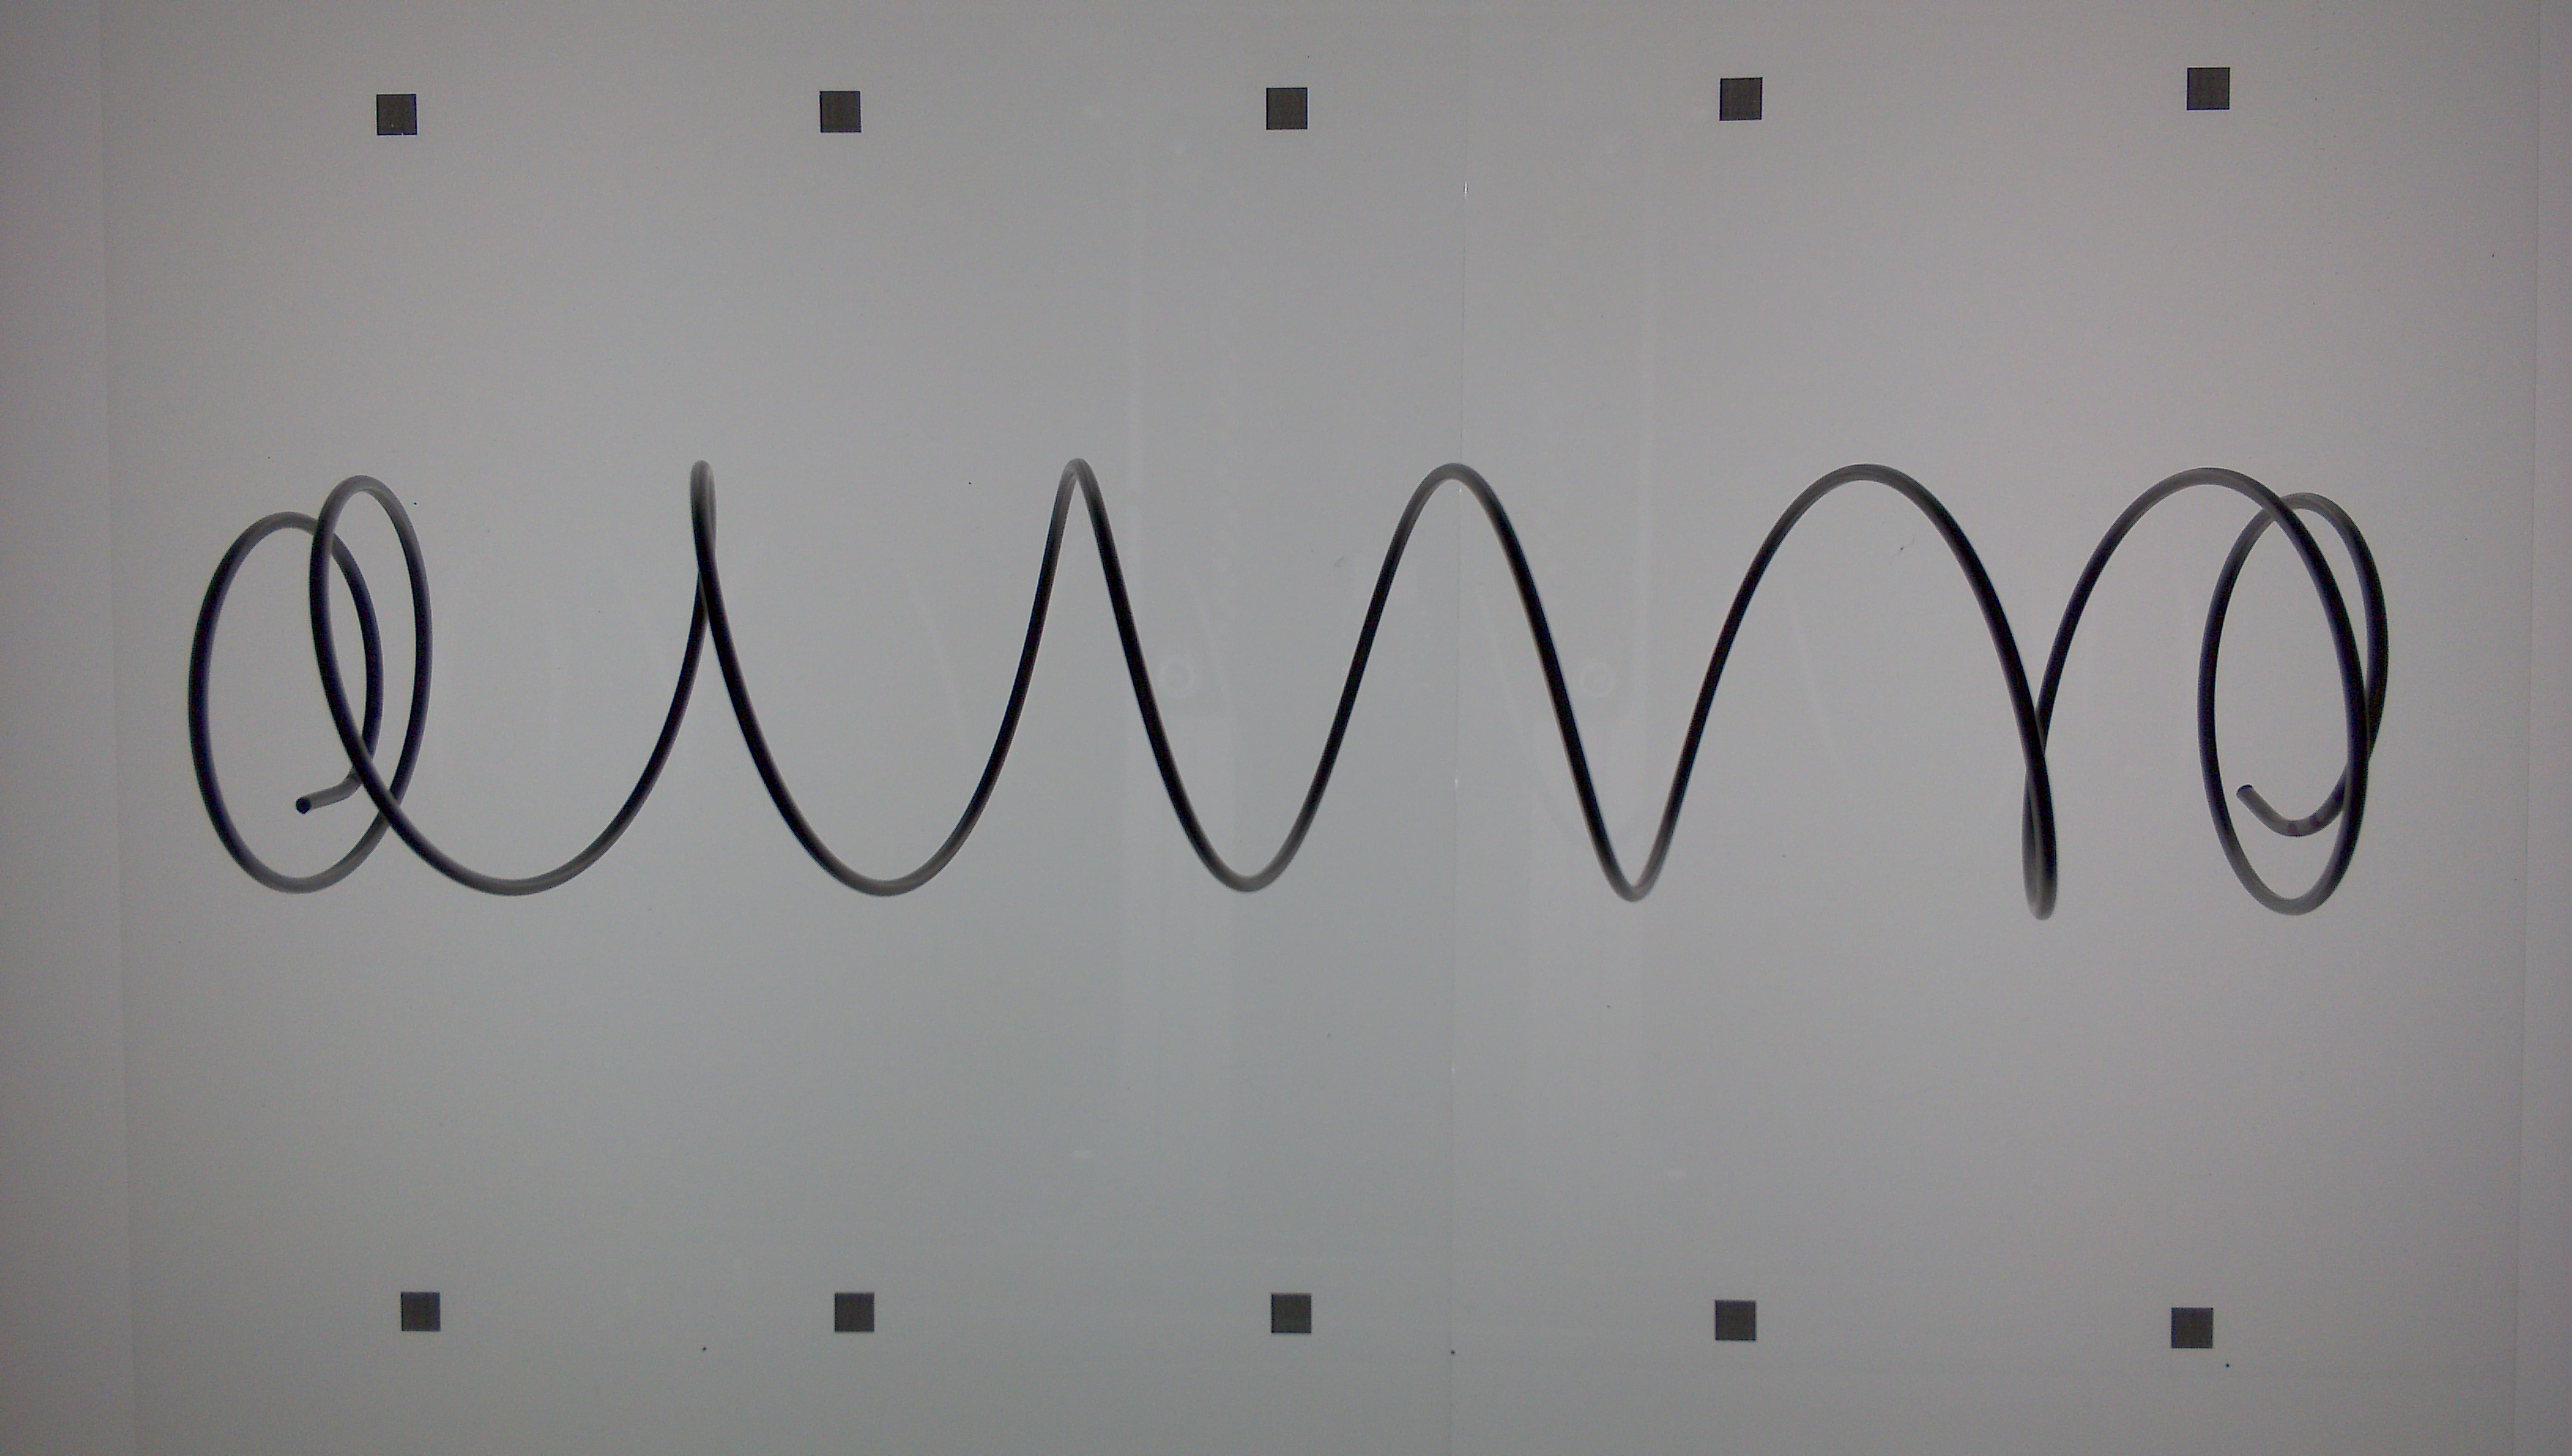
\includegraphics[width=150pt]{bim1.png} at (0,0);

	\node[inner sep=0pt] (russell) at (0,0)
	{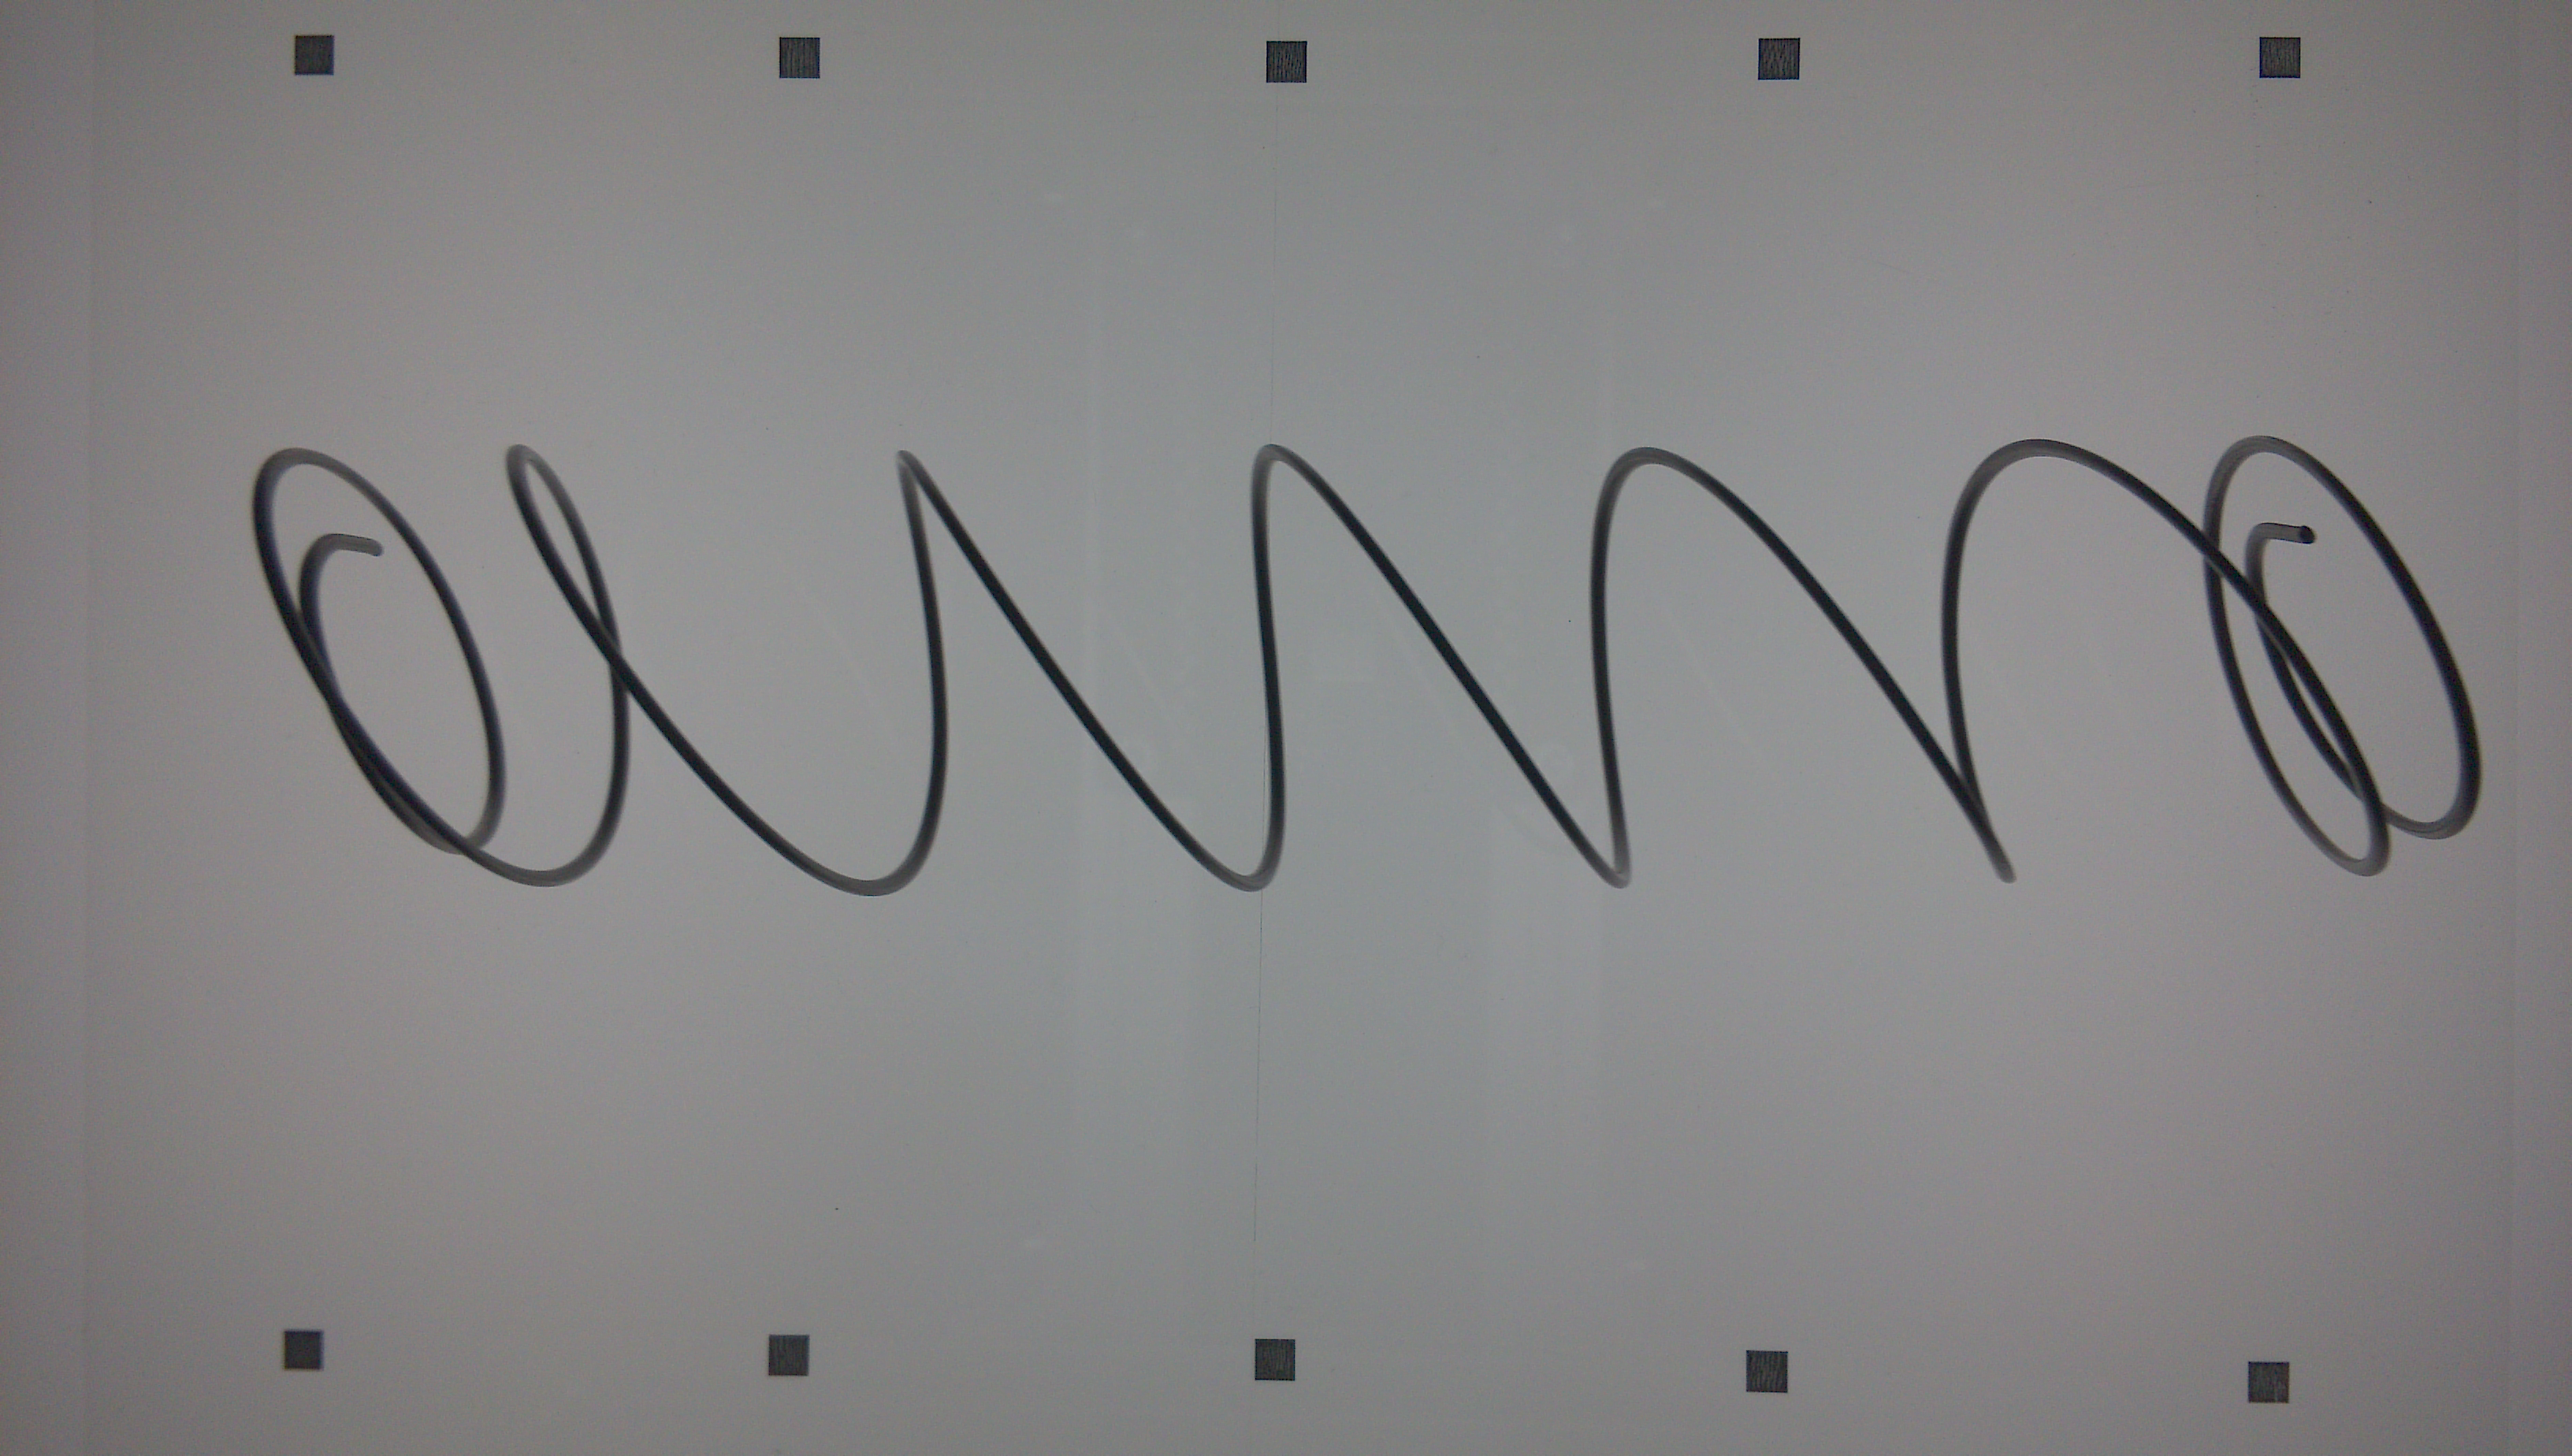
\includegraphics[width=10cm, height=6cm]{rolling.png}};
	\draw[color = blue , thick] (-4.02,-0.7)--(4.67,-0.7);
	\draw[color = blue , thick] (-4.02,1.2)--(4.67,1.2);

	\draw[color = blue , thick ] (-4.02,-0.7)--(-4.02,1.2);
	
	\draw[color = blue, thick  ] (4.67,-0.7)--(4.67,1.2);

	\draw[<->,color = black!10!white](-4.02,-1.2)-- node[below]{Distorted length trough rolling shutter}(4.67,-1.2);
	\draw[<->,color = black!10!white](-4.5,-0.7)-- node[above, rotate= 90]{Undistorted diameter}(-4.5,1.2);
	
	\end{tikzpicture}
\end{document}	